% Options to documentclass:
% . Preprint: default option
% . Review: increases line spaces
% . 1p: 1+ journals with a text area of 13.5cm ×19.75cm, single column style
% only.
% . 3p: 3+ journals with a text area of 16.45cm ×21.9cm, single column style.
% . 5p: 5+ with text area of 18.35cm ×24cm double column style only.
% . twocolumn: should be used along with 3p option if the journal is 3+ with
% the same text area as above, but double column style.
\documentclass[review]{elsarticle}

\usepackage{lipsum} % Fill lorem ipsum text

\usepackage{lineno} % Line numbers
\modulolinenumbers[1] % Frequency to print line numbers
\usepackage{hyperref} % Hyperlinks
\hypersetup{ % Configuration of hyperlinks
    colorlinks=true,
    linkcolor=blue,
    filecolor=magenta,
    urlcolor=cyan,
    pdftitle={ARTICLE TITLE},
    pdfauthor={AUTHOR},
}

% Draw plots (normally done in a separate file, to improve compilation time)
\usepackage{pgfplots}
\pgfplotsset{compat=1.17}
\usepgfplotslibrary{units} % Include units in axis
\usepackage{graphicx} % Enhanced graphics support
\usepackage[dvipsnames]{xcolor} % Enhanced color support

\usepackage{subcaption} % Makes subfigure and subtable environments available
\usepackage{booktabs} % Draw tables
\usepackage{multirow} % Makes multirows available in tables

% Write algorithms in pseudocode format
\usepackage{algorithm}
\usepackage{algorithmic}

% Additional mathematical symbols
\usepackage{amsmath}
\usepackage{amssymb}
\usepackage{mathtools}
\usepackage{bm} % Bold math symbols

\usepackage{newtxtext,newtxmath} % New text and math font

% Definition of the bibliographic style and the .bib file
\usepackage[backend=biber, style=apa, citestyle=apa]{biblatex}
\addbibresource{mybib.bib}

\journal{JOURNAL NAME}

\begin{document}

\begin{frontmatter}

\title{ARTICLE TITLE}

\author[firstAddress,secondAddress]{AUTHOR 1\corref{correspAuthor}}
\ead{AUTHOR_1@EMAIL.com}

\author[secondAddress]{AUTHOR 2}

\address[firstAddress]{FIRST ADDRESS}
\address[secondAddress]{SECOND ADDRESS}
\cortext[correspAuthor]{Corresponding author}

\begin{abstract}
    \lipsum[2-3]
\end{abstract}

\begin{keyword}
    KEYWORD 1 \sep{} KEYWORD 2 \sep{} KEYWORD 3 \sep{} KEYWORD 4
\end{keyword}

\end{frontmatter}

\linenumbers{}

\newcommand{\uu}[1]{\underline{\underline{#1}}}
  \section*{List of Symbols}
  \begin{tabular}{l{0.5cm}l{7cm}}
    $\uu{\sigma}$ &Second rank stress tensor\\
    $\sigma_{eq}$ &Von Mises equivalent stress \\
    $f_{y}$       &Yield stress \\
    $\uu{s}$      &Second rank deviatoric stress tensor \\
    $J_{2}$       &Second invariant of the deviatoric stress tensor\\
    $J_{3}$       &Third invariant of the deviatoric stress tensor\\

    \multicolumn{2}{c}{} \\

    $p$                          &Equiv. creep (viscoplastic) strain \\
    $\uu{\dot \varepsilon}^{cr}$ &Second rank creep (viscoplastic) strain
    rate tensor\\

    \multicolumn{2}{c}{} \\

    $A$, $n$, $m$          &Temperature dependent isotropic creep parameters \\
    $w$                    &Weights \\

    \multicolumn{2}{c}{} \\

    $e$           &Sample's thickness \\
    $\phi_s$      &Sample's diameter \\
    $\phi_j$      &Jaws' diameter \\

    \multicolumn{2}{c}{} \\

    $\uu{I}$      &Identity matrix \\
    $Tr()$        &Trace \\
    $\left\langle \quad \right\rangle$  &Macaulay brackets \\
    $x^{\pm}$  &Positive and negative parts of variable $x$\\

    \multicolumn{2}{c}{} \\

    $F$  &Force \\
    $t$  &Time \\
  \end{tabular}

\section{Introduction}\label{sec:intro}

\lipsum[2-5]

This is a citation \parencite{teixeira2021}.

This is a in-text citation, according to \textcite{teixeira2020}.

\section{Section 2}\label{sec:section2}

\lipsum[2-4]

\subsection{Subsection title}\label{subsec:title}
\lipsum[2-2]
\subsubsection{Subsubsection title}\label{subsubsec:title}
\lipsum[3-3]
\paragraph{First paragraph}
\lipsum[4-4]
\paragraph{Second paragraph}
\lipsum[5-5]

\section{Section title}\label{sec:section3}

Reference to Figure~\ref{fig:plot}.

\begin{figure}[hbt!]
  \centering
  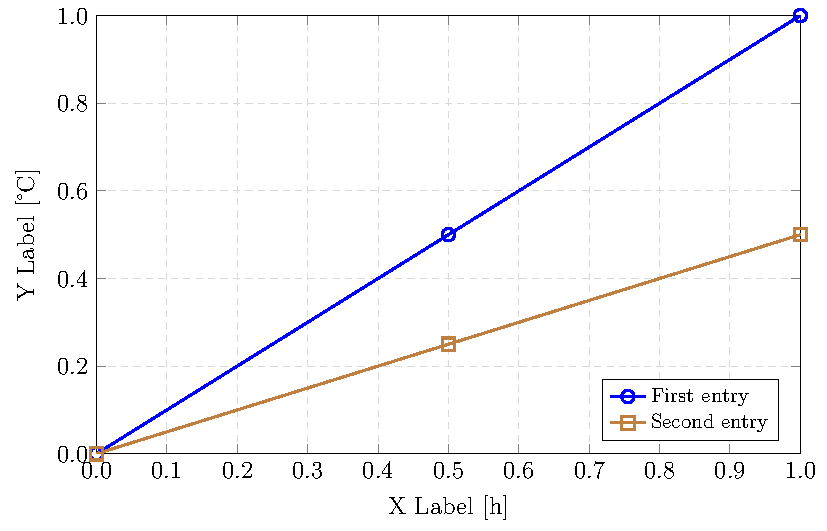
\includegraphics[width=0.8\linewidth]{figures/plot1.pdf}
  \caption{Figure caption}\label{fig:plot}
\end{figure}

This is a reference to Figure~\ref{fig:subfig}, which is divided into
Figure~\ref{fig:subfig-a} and Figure~\ref{fig:subfig-b}.

\begin{figure}[hbt!]
  \centering
  \begin{subfigure}[c]{0.49\textwidth}
    \centering
    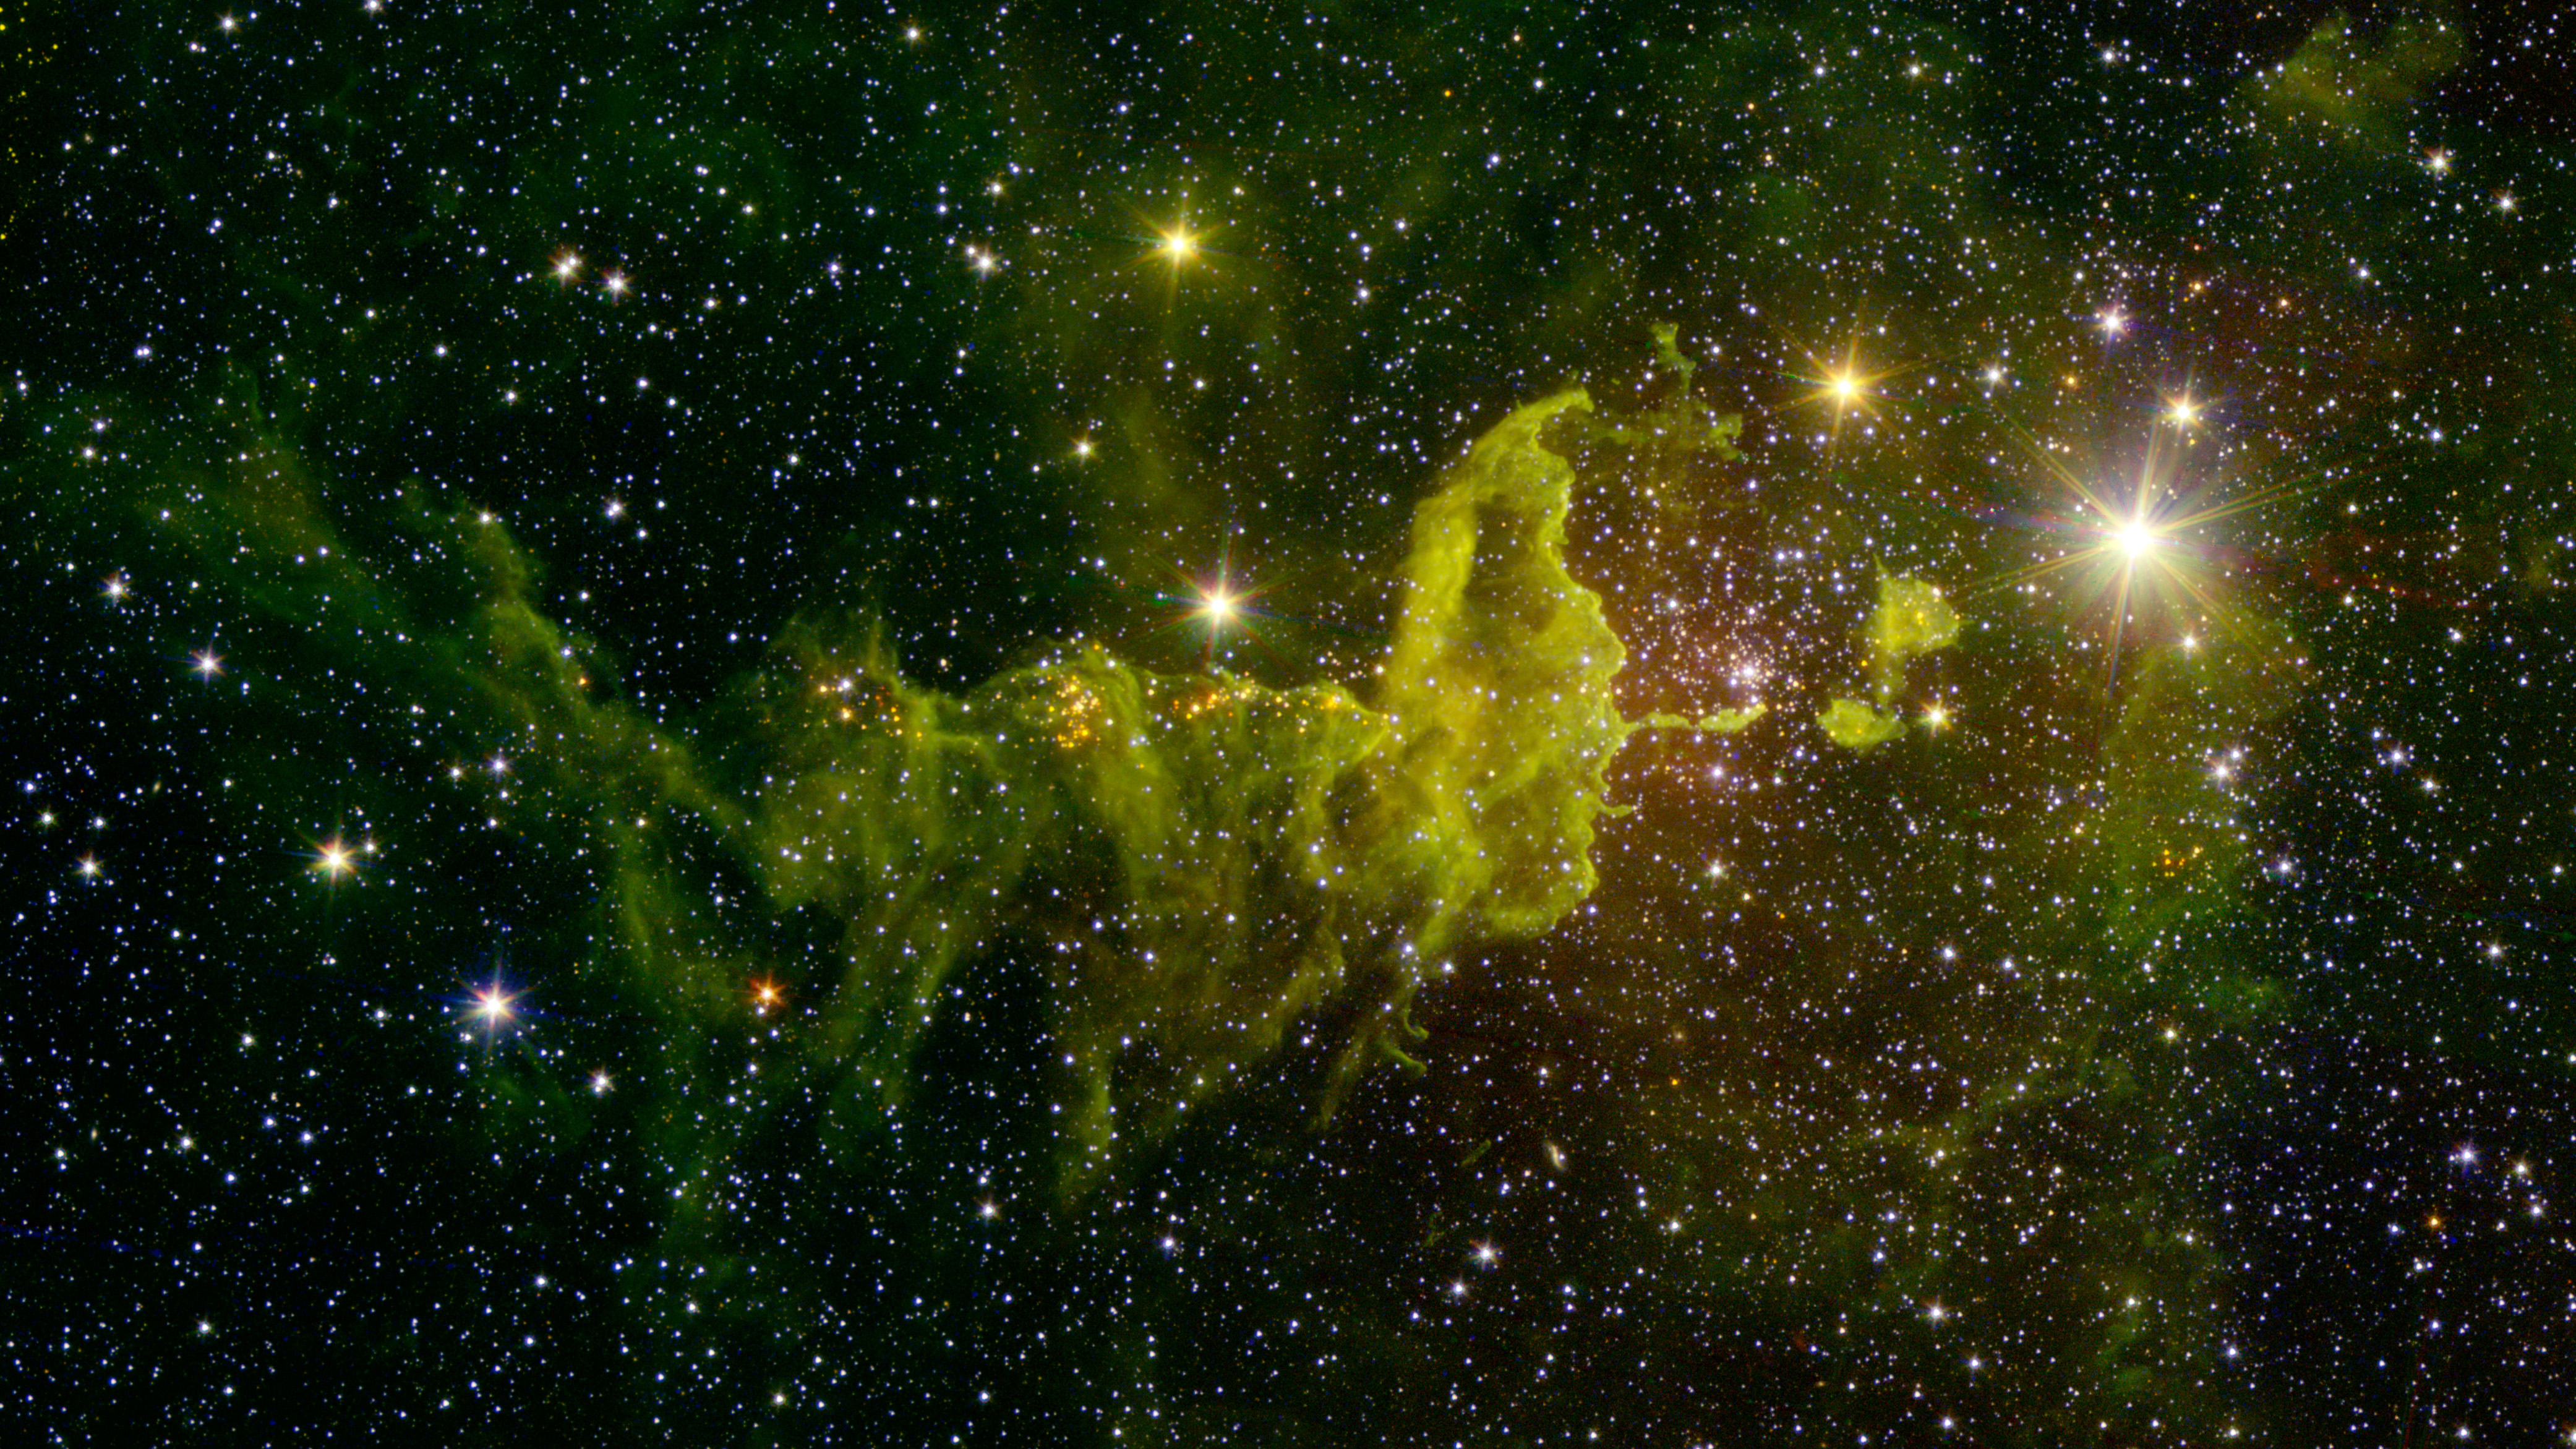
\includegraphics[width=\linewidth]{figures/figure1.jpg}
    \caption{}\label{fig:subfig-a}
  \end{subfigure}
  \begin{subfigure}[c]{0.49\textwidth}
    \centering
    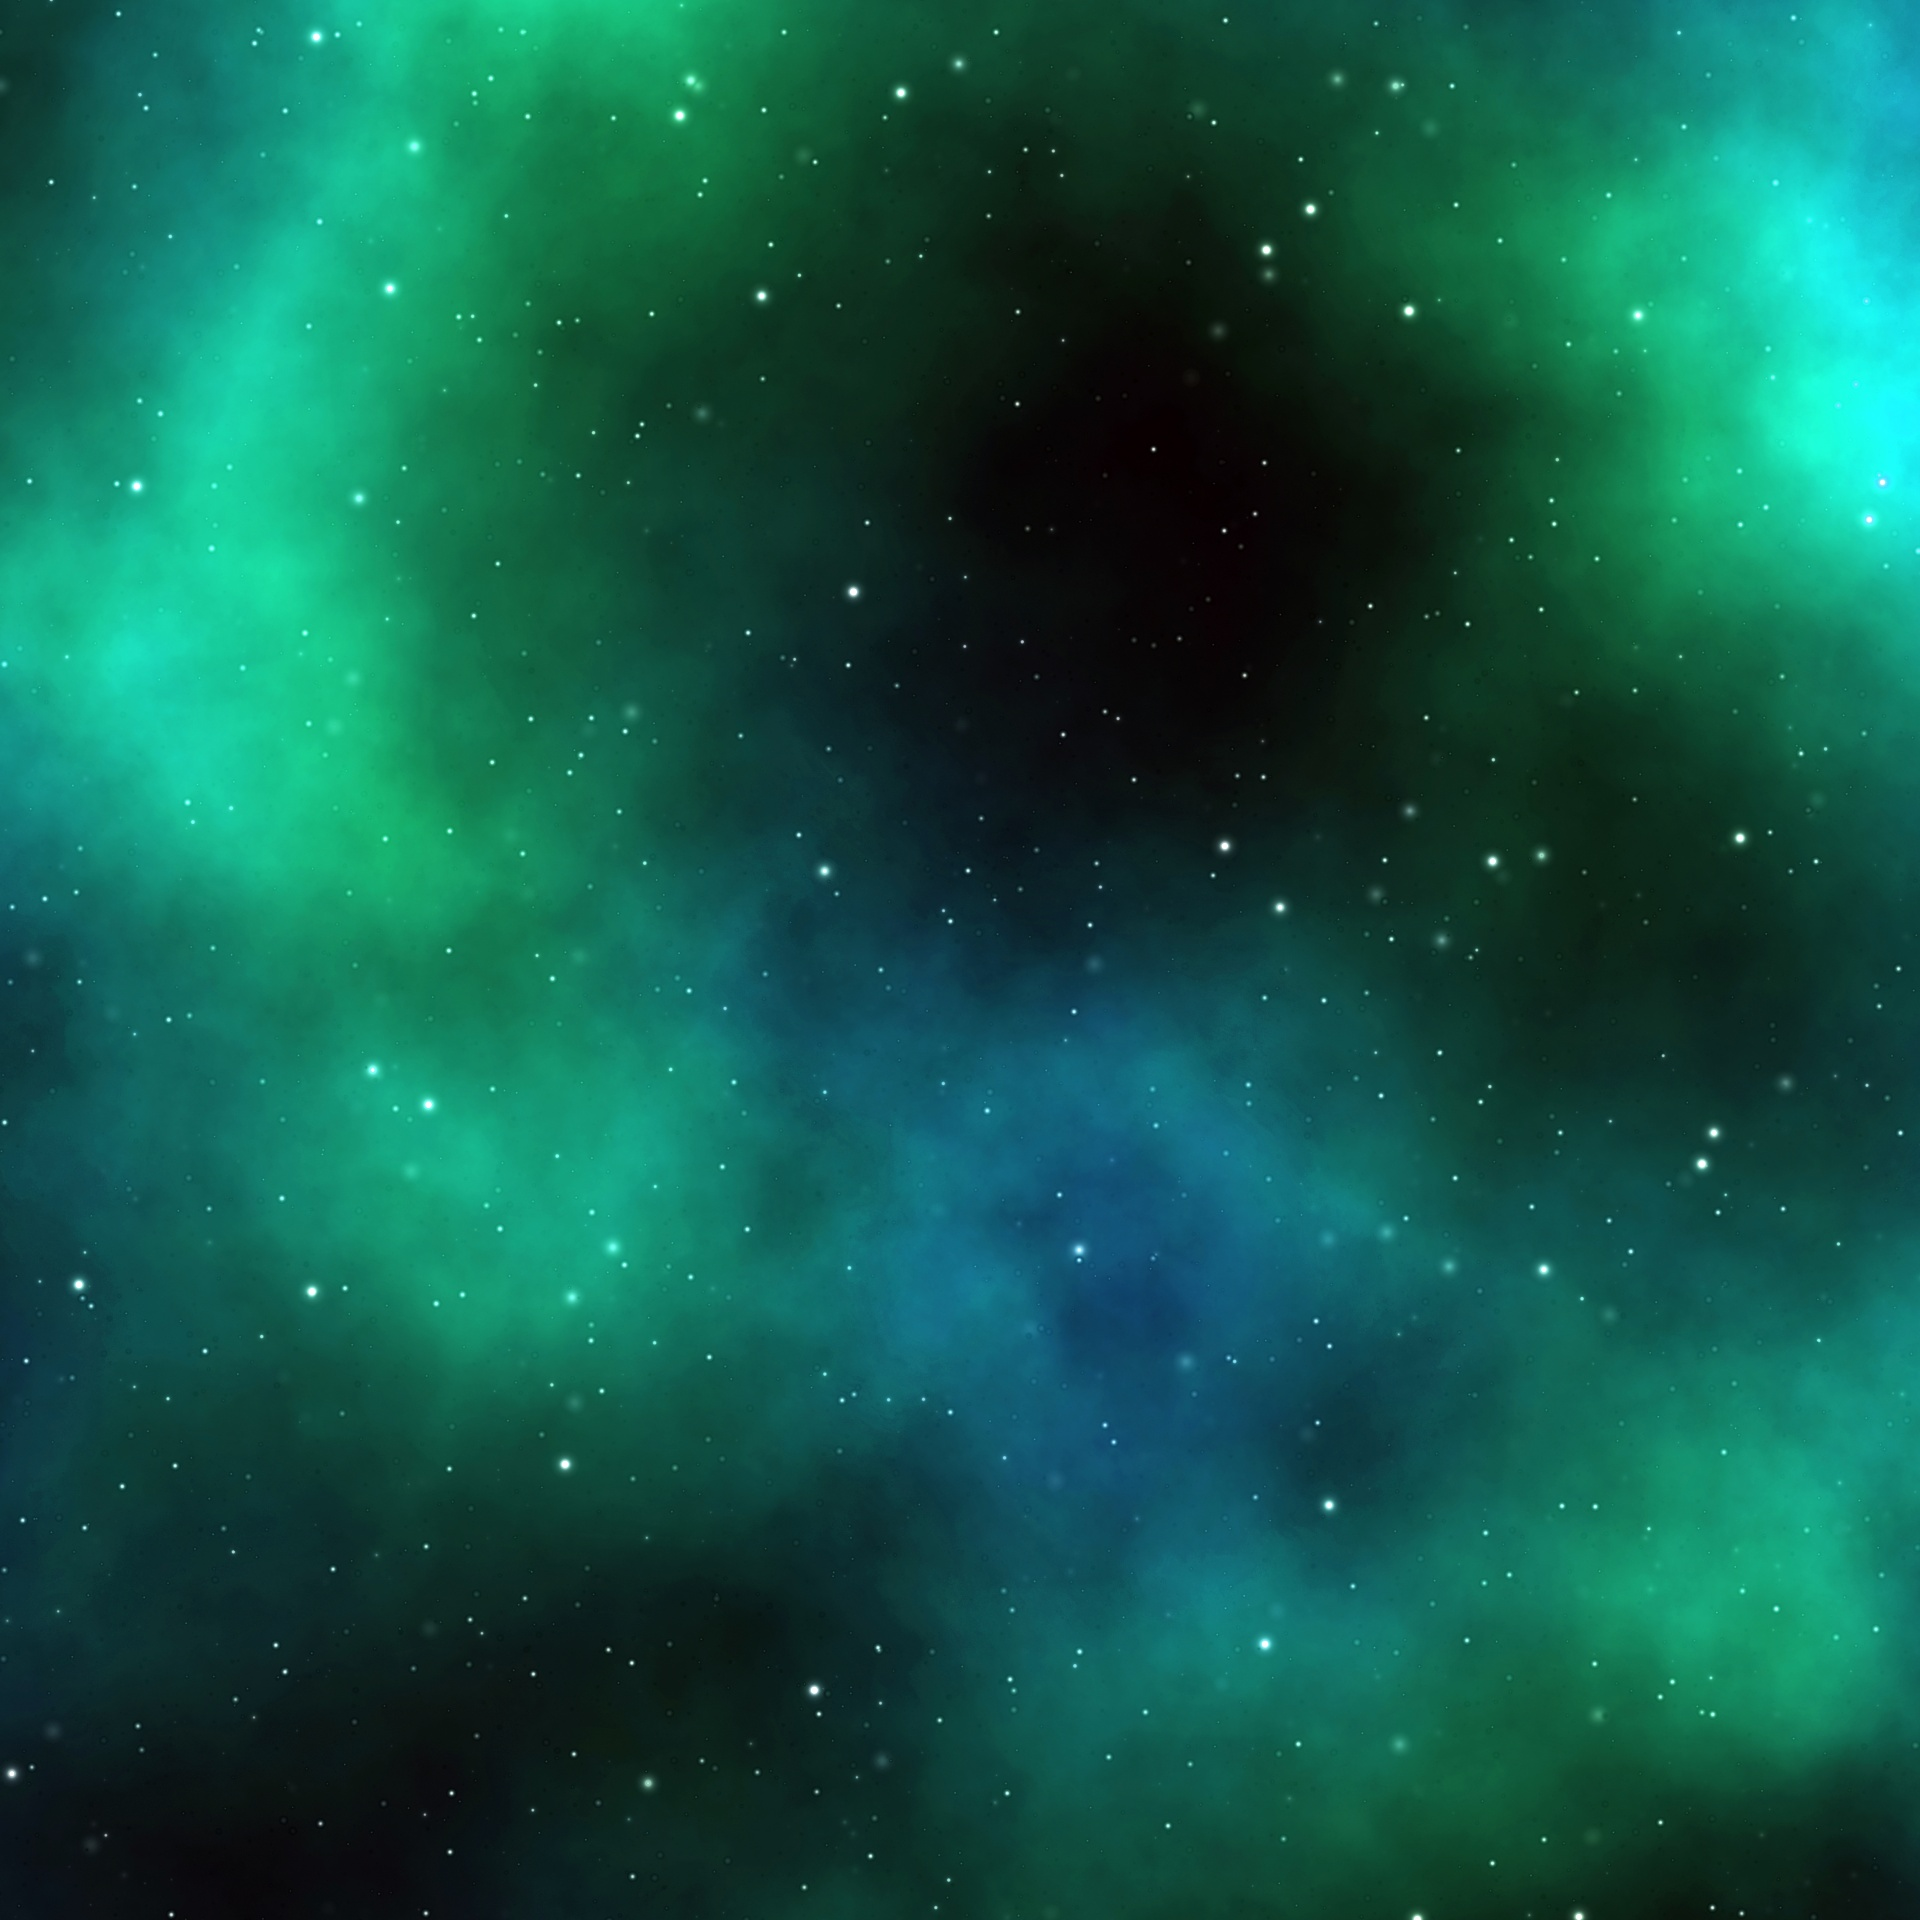
\includegraphics[width=\linewidth]{figures/figure2.jpg}
    \caption{}\label{fig:subfig-b}
  \end{subfigure}
  \caption{Figure with subfigures}\label{fig:subfig}
\end{figure}

Reference to Table~\ref{tab:table}.

\begin{table}[hbt!]
  \centering
  \renewcommand{\arraystretch}{1.1}
  \caption{Table caption}
  \begin{tabular}{p{0.3\linewidth}c{0.12\linewidth}c{0.12\linewidth}}
   \toprule
   \textbf{Column 1} & \textbf{Column 2} & \textbf{Column 3} \\
   \midrule
   Description 1 & 0.1 & 1.0 \\
   Description 2 & 0.2 & 2.0 \\
  \bottomrule
  \end{tabular}\label{tab:table}
  \renewcommand{\arraystretch}{1}
\end{table}

Reference to Equation~\ref{eq:relativity}.

\begin{equation}
\label{eq:relativity}
   E = mc^{2}
\end{equation}

\section{Conclusion}\label{sec:conclusion}

\lipsum[10-10]

\section*{Acknowledgments} This work was supported by the funding scheme of the
FUNDER, in the frame of the project PROJECT, grant number 123456.


\printbibliography{}

\end{document}
